\documentclass[11pt,a4paper]{article}

\usepackage[margin=1in]{geometry}
\usepackage{hyperref}
\usepackage{enumitem}
\usepackage{parskip}
\usepackage{pdfpages}

\title{CS5013 Project Proposal \\ \large\textit{BibMerge: Automated Deduplication and
Merging of BibTeX References Across Papers}}
\author{S Naveen, CS26E010 \and Gowni Vamshi, CS26E005}
\date{\today}

\begin{document}
\maketitle

\section{Team information}

Team ID: CS26E010.

\begin{itemize}[nosep]
  \item Member 1: S Naveen -- roll no. CS26E010 -- department CSE
        -- GitHub handle Sajjan-Naveen-87
  \item Member 2: Gowni Vamshi -- roll no. CS26E005 -- department CSE
        -- GitHub handle vamshiG24
\end{itemize}

Primary contact email: cs26e010@smail.iitm.ac.in.

\section{Problem statement}

Researchers routinely work across many academic papers, and each paper
carries its own \texttt{.bib} bibliography. When these bibliographies are
combined -- for a survey, a thesis, or a shared group library -- the same
cited work often appears more than once under different citation keys and
with inconsistently formatted fields, so merging them by hand is slow and
error-prone. The pain is concrete: the researcher must open several
\texttt{.bib} files side by side, visually spot that two differently
labelled entries are in fact the same paper, and manually reconcile them,
repeating the whole check every time a new paper is added. This is the
stakeholder's problem as a working researcher who accumulates and reuses
references across projects. There is currently no automated way to map
duplicate references to a single canonical entry and keep that mapping
consistent as new papers arrive.

\section{Users and stakeholder}

Named stakeholder: Ashrujit Ghoshal, Assistant Professor,
Department of Computer Science and Engineering, IIT Madras
(ashrujit@cse.iitm.ac.in).

We first spoke with Dr.\ Ghoshal on 18 August 2026 about the recurring
difficulty of managing overlapping bibliographies when writing and
combining research papers, and followed up by email the same day. On
19 August 2026 he asked us to write down the points discussed as a formal
problem statement, which we did, and on 20 August 2026 he confirmed it with
``Sounds good.'' The problem he described: when references from multiple
papers are brought together, the same cited work frequently appears under
different BibTeX keys and formatting, and deduplicating them by hand is
tedious and easy to get wrong. He agreed that an automated tool to parse,
deduplicate, and merge \texttt{.bib} files -- and to keep a stable
canonical entry as further papers are imported -- would be useful to him
and to others in his group.

The stakeholder's acknowledgement email is attached as Appendix~A.

\section{Prior work and why it does not suffice}

\begin{enumerate}[leftmargin=*]
  \item \textbf{JabRef} -- \url{https://www.jabref.org}.
        Overlap: an open-source BibTeX reference manager that parses
        \texttt{.bib} files and includes a ``Find duplicates'' feature that
        detects and merges duplicate entries.
        Gap: it is an interactive desktop application built to curate a
        single personal library, not a scriptable batch pipeline for
        merging many papers' \texttt{.bib} files against a persistent
        canonical set. Duplicate resolution is manual and one pair at a
        time, and there is no notion of incrementally re-importing a new
        paper and automatically mapping its references to already-merged
        entries.
  \item \textbf{BibTool} --
        \url{http://www.gerd-neugebauer.de/software/TeX/BibTool/}.
        Overlap: a command-line tool for manipulating BibTeX databases that
        can normalise entries and remove duplicate citation keys.
        Gap: it detects duplicates by citation key or exact field matches,
        not by semantic identity. Two entries for the same paper with
        different keys and slightly different fields are not recognised as
        the same work; there is no fuzzy or identifier-based (DOI) matching
        and no persistent duplicate-to-canonical mapping.
  \item \textbf{Zotero / Mendeley} -- \url{https://www.zotero.org}.
        Overlap: reference managers that import references, flag
        ``Duplicate Items,'' and merge them.
        Gap: both are GUI, library- and account-centric tools. Importing
        and exporting BibTeX round-trips through their internal data model,
        which reformats or drops fields, and they are not designed to take
        a set of per-paper \texttt{.bib} files and emit one clean merged
        \texttt{.bib}. They are heavier and more cloud-oriented than the
        stakeholder's workflow needs.
  \item \textbf{Manual copy-paste (the current incumbent)} -- internal /
        manual.
        Overlap: the researcher opens each paper's \texttt{.bib}, copies
        entries into one file, and eyeballs the result for duplicates.
        Gap: this is exactly the slow, error-prone process the project
        aims to replace; it does not scale as the number of papers grows
        and must be redone from scratch whenever a new paper is added.
\end{enumerate}

\section{Tech stack}

Language: \textbf{Java} (course policy). The core parsing,
deduplication, and merging engine -- all of the project's logic -- is
written in Java; the React/TypeScript layer is only the browser front end
that calls it.

The tool is delivered as a \textbf{web application}: a React + TypeScript
single-page front end talking to a Java (Spring Boot) REST back end that
performs the BibTeX processing.

\begin{itemize}[nosep]
  \item Build system: \textbf{Maven} for the Java back end (reproducible
        build producing a runnable JAR); \textbf{npm + Vite} for the React
        front end.
  \item Framework: \textbf{Spring Boot} (Spring Web REST API) on the back
        end; \textbf{React} with \textbf{TypeScript} (Vite) on the front
        end.
  \item Key libraries:
        \textbf{JBibTeX} (parse and format BibTeX);
        \textbf{Apache Commons Text} (Levenshtein / Jaro--Winkler string
        similarity for fuzzy matching);
        \textbf{Spring Boot Web} (REST endpoints for upload, merge, and
        download);
        \textbf{JUnit~5} (back-end testing);
        \textbf{React + Vite + TypeScript}, with \textbf{Axios} for the
        front-end API calls.
  \item Where the tool will run: as a web app -- the Spring Boot service
        runs on the stakeholder's machine or a department server, and the
        stakeholder uses it from a browser to upload \texttt{.bib} files,
        review matches, and download the merged bibliography.
\end{itemize}

\section{AI-usage statement}

\textit{%
We will use AI coding assistants (such as Claude Code, GitHub Copilot,
ChatGPT, or Gemini) during this project, in line with the course
policy on AI-assisted programming.
Every line of code we submit will be code we understand and can
explain in the viva, whether we typed it or the assistant generated
it.%
}

\section{Verification plan}

Test fixtures we will use:

\begin{itemize}[nosep]
  \item A de-identified sample of \texttt{.bib} files taken from three to
        five of the stakeholder's own papers, containing real
        cross-paper duplicate citations.
  \item A synthetic corner-case set covering: two entries with the same DOI
        but different citation keys; title, whitespace, casing, and
        diacritic variants of the same reference; entries with missing
        fields; duplicate keys within a single file; and empty / malformed
        input files.
\end{itemize}

User-visible acceptance criteria the stakeholder will use to say
``yes, this works'':

\begin{itemize}[nosep]
  \item Merges the \texttt{.bib} files from several of the stakeholder's
        papers into a single file containing no duplicate entries, matching
        a hand-checked reference merge.
  \item Correctly recognises two differently labelled entries for the same
        paper as one canonical entry (matched first by DOI, then by fuzzy
        title/author/year), rather than emitting both.
  \item Re-importing an already-merged paper adds zero new duplicate
        entries and maps its references onto the existing canonical set.
  \item Produces a valid \texttt{.bib} file that compiles under
        BibTeX/biblatex without errors.
\end{itemize}

\section{Milestone plan}

\begin{itemize}[nosep]
  \item \textbf{By the design doc (11 Sep 2026):}
        scope locked; the Spring Boot back end and the React + TypeScript
        front end scaffolded; JBibTeX parsing an uploaded \texttt{.bib}
        file into an internal reference model; the matching strategy
        (DOI-first, then fuzzy) prototyped on a small sample.
  \item \textbf{By the mid-demo (9 Oct 2026):}
        the core workflow running end-to-end through the web app -- upload
        two or more real \texttt{.bib} files from the stakeholder's papers,
        deduplicate and merge them on the back end, and download a single
        merged \texttt{.bib}.
  \item \textbf{By the final submission (6 Nov 2026):}
        the stakeholder can use the deployed web app themselves to merge a
        set of papers and to incrementally import new papers, reviewing a
        report of merged and uncertain matches in the browser.
\end{itemize}

\section{Risks and plan B}

\begin{enumerate}[leftmargin=*, nosep]
  \item \textbf{Risk:} many references lack a DOI or other stable
        identifier, so exact matching is impossible.
        \textbf{Plan B:} fall back to normalised fuzzy matching on
        title, author, and year, and surface uncertain matches in a review
        report instead of merging them silently.
  \item \textbf{Risk:} a false merge collapses two genuinely distinct
        papers into one, losing a reference.
        \textbf{Plan B:} use conservative similarity thresholds with a
        human-confirmation step for borderline matches; never discard data
        -- keep an audit log of every merge decision.
  \item \textbf{Risk:} BibTeX in the wild varies widely (biblatex vs.\
        classic BibTeX, non-standard fields, encoding and diacritic
        issues).
        \textbf{Plan B:} document a clearly supported subset/schema, ship a
        normaliser for common variants, and preserve unknown fields
        verbatim on output so nothing is lost.
\end{enumerate}

\appendix
\renewcommand{\thesection}{Appendix~\Alph{section}}

\section{Stakeholder acknowledgement email}\label{app:email}

The stakeholder's acknowledgement is the email thread ``Request for
Collaboration: CS5013 Course Project Stakeholder'' (IIT Madras Mail). The
acknowledgement is the final message from Ashrujit Ghoshal, dated
20 August 2026 (``Sounds good''). The original PDF is included in full on
the following pages.

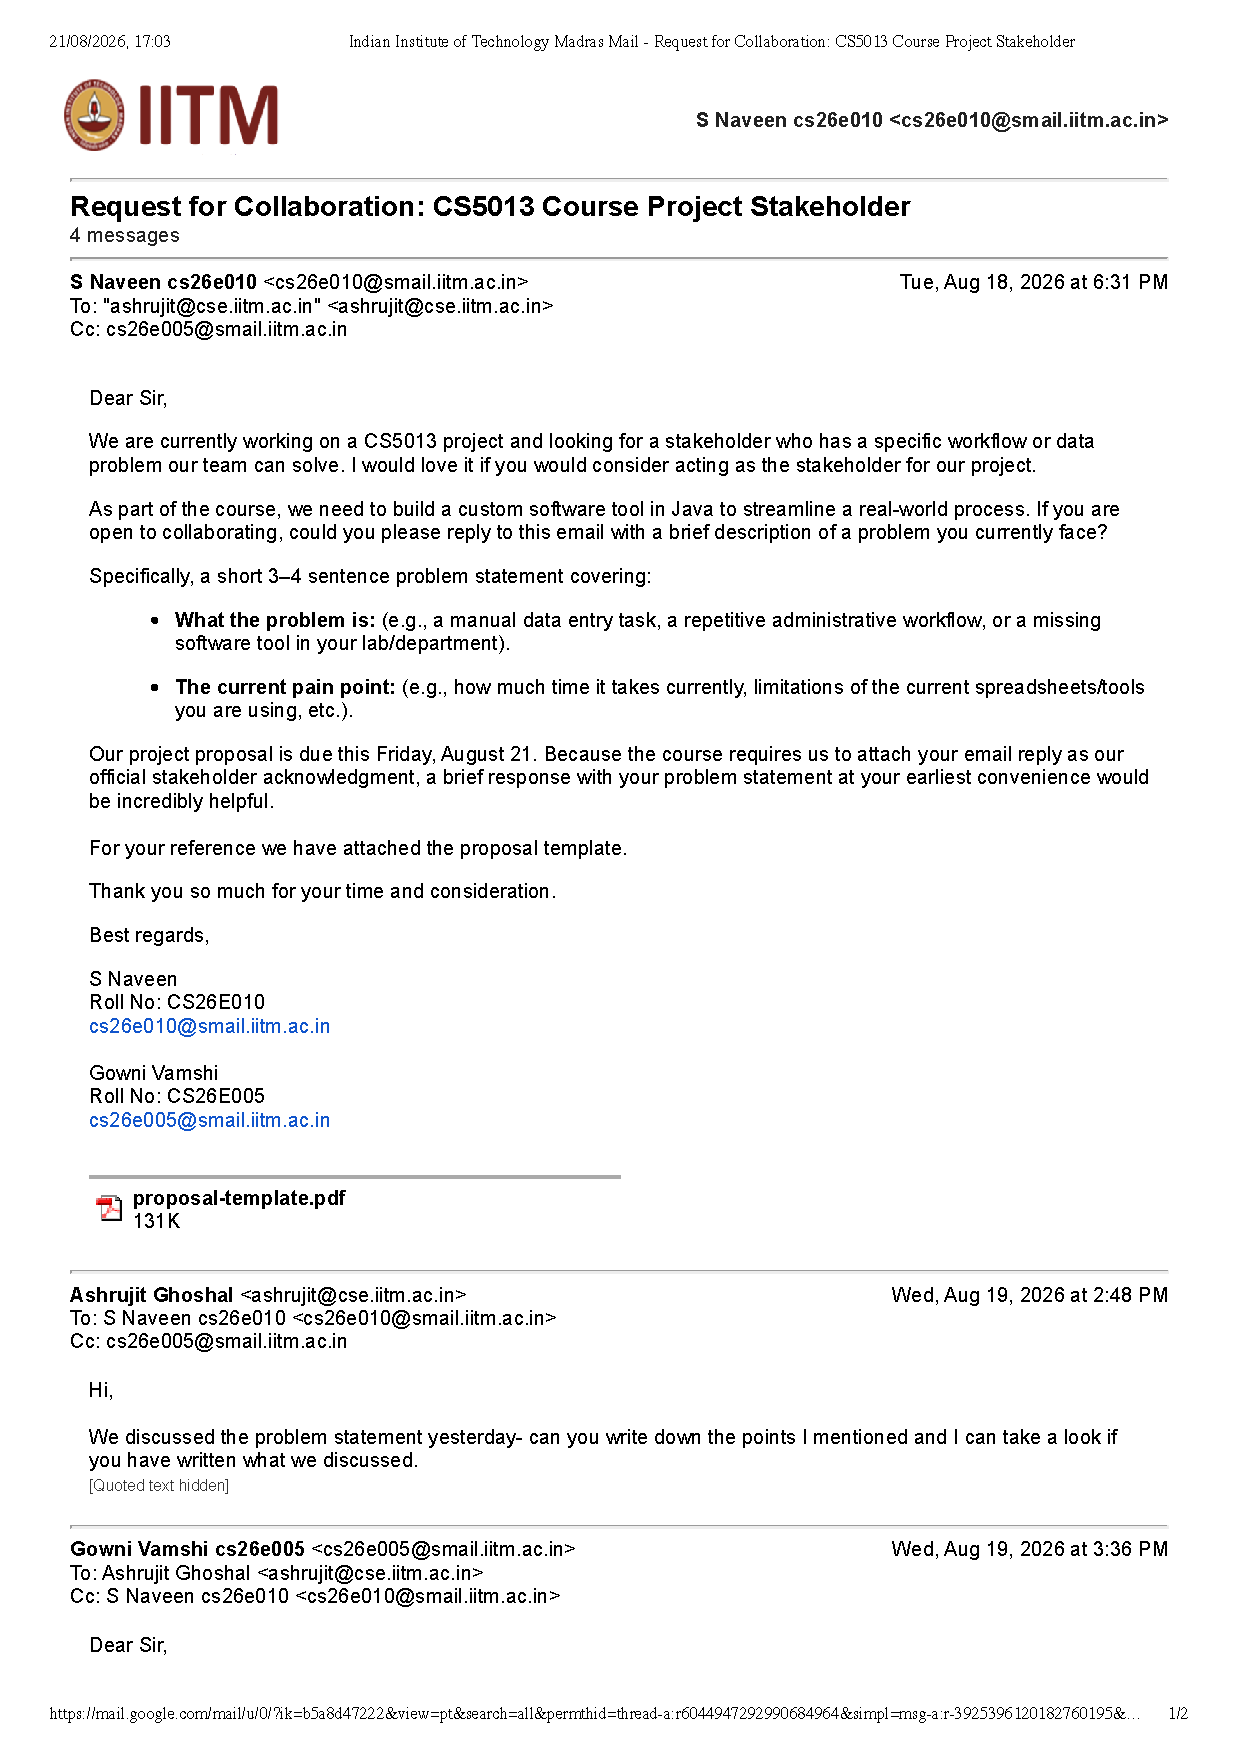
\includepdf[pages=-]{stakeholder-email.pdf}

\end{document}
